\documentclass[12pt]{article}
\usepackage[english]{babel}
\usepackage[utf8x]{inputenc}
\usepackage{amsmath}
\usepackage{graphicx}
\usepackage[colorinlistoftodos]{todonotes}
\usepackage{listings}
\usepackage{hyperref}
 
\hypersetup{
 colorlinks=true,
 linkcolor=blue,
 filecolor=magenta, 
 urlcolor=cyan,
}
 
\lstset{
 basicstyle=\ttfamily,
 columns=fullflexible,
 breaklines=true,
 postbreak=\mbox{\textcolor{red}{$\hookrightarrow$}\space},
}
 
\begin{document}
\begin{titlepage}
	\centering
	{\scshape\Huge\textbf{Keep your distance}\par}
	\vspace{1cm}
	{\scshape\Large Internet of Things - Project Report\par}
	\vspace{2cm}
	{\scshape\Large\emph{Sergio Cuzzucoli 10532314}\\ \emph{Daniele De Dominicis 10502843}\par}
	\vspace{4cm}
	{\scshape\normalsize{June, 2021}}
\end{titlepage}


\section{Data structures}

\subsection{Message}
Each mote exchanges a message composed only of the sender ID. In particular the sender Id is a 16 bits unsigned integer; this allows us to have up to \(2^{16}-1\) IDs.

\subsection{Contacts}
Each mote keeps track of the other motes currently in its range through a structure that contains:
\begin{itemize}
  \item \textbf{id}, id of the mote in range stored as 16 bits unsigned integer;
  \item \textbf{timeStamp}, indication of time of the last message sent by said mote stored as 32 bits unsigned integer;
  \item \textbf{counter}, with values in range [1,10] stored as 8 bits unsigned integer.
\end{itemize}

\section{Basic functioning of the mote}
Each mote broadcasts a message every 500ms.\newline
When two motes come in contact they exchange messages and the receiving mote starts to populate its contact list with all the information of the sender.\newline
If the two motes continue to exchange packets every 500ms then the counter of the respective contacts is increased by 1 every time. When the counter reaches the value of 10, the mote sends an "Alarm message" signaling that it has been in contact for too much time with the mote.\newline
We assume that one mote will not communicate, at least at the same time, with all the other motes, thus the list of contact has a fix length which is lower than the number  of possible motes.
This is the reason behind the fact that the list is updated every firing of the timer to send the message.\newline
Before sending a message every mote checks every entry in its contact list: if the difference between the current value of the timer and the timestamp of the last message received is grater than 500ms, then the mote has not received any keep-alive from the contact in 500ms. In this case we realize that the two motes went out of range and thus there is no need to keep the information about the contact.


\section{From Cooja to NodeRed}
Each mote prints a message that is shown in Cooja and forwarded to NodeRed.

\section{NodeRed}

In NodeRed, nodes stay alway up listening for messages sent by motes. Such messages converge into a single node which will route them according to its type.

\subsection{General log flow}
Every message is sent to another node which will remove the impurity, constituted by random characters injected at the beginning of the message by cooja. A timestamp of the in the format [YY/MM/DD HH:MM:SS] is then added at the beginning.Finally, the resulting lines are appended to a txt file which will work as the log file of the application.

\subsection{Alarm message flow}
In addition to being stored in the log files, ALARM messages have also to be sent to the user via IFTTT. \newline
First of all they undergo a process which removes the impurity at the beginning and extracts the motes ID, then these IDs are passed through a POST request via parameters of the URL at our IFTTT Applet.

\section{IFTTT}
The behavior of the Applet is quite simple:
\begin{itemize}
  \item{\textbf{IF-THIS side:} the Applet exposes a webhook, in order to receive the IDs from NodeRed.
  \item {\textbf{THAN-THAT side:} once triggered by the reception of a message from NodeRed, the applet sends a message to the Telegram account of the IFTTT account owner.}}
\end{itemize}

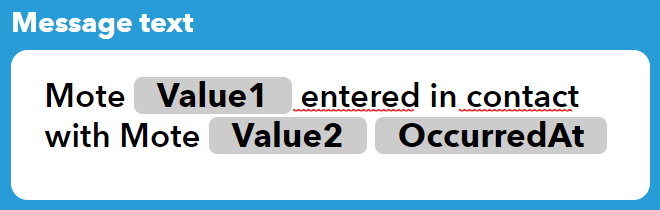
\includegraphics[scale=0.8]{Message_Text.PNG}

\section{Log}

Logs file store five types of messages:
\begin{enumerate}
\item \textbf{[START:X]} Mote X has correctly started;
\item \textbf{[RANGE:X/Y]} Mote X has come in contact with mote Y;
\item \textbf{[UPDATE:X/Y-N]} Mote Y is still in range of mote X and it has sent the N-th message (with N which can have values between 2 and 10);
\item \textbf{[OUT:X/Y]} Mote Y is no longer in the range of mote Y.
\item \textbf{[ALARM:X/Y]} Mote X has sends an Alarm to the owner, after being in range with Mote Y for 5 seconds.
\end{enumerate}

\section{Demonstration}
In our simulation we have considered 5 motes. First of all they are turned on. Then Mote 1 goes in range with Mote 2 exchanging 7 consecutive messages, after that Mote 2 goes out of range. Again Mote 1 goes in range with Mote 2 until the alarm is sent by both Motes; in the end they go out of range. In the mean time Motes 3, 4 and 5 goes in range between each others, sending the Alarms. Next they go out of range.

\end{document}